% !TEX root = ../../../proposal.tex

\section{Variational Autoencoders and Disentangled Representations}
\label{sec:vae_disentanglement}

\subsection{The Variational Autoencoder}

A standard autoencoder can learn a compact code that reconstructs an input, but it does
not guarantee that the code space is useful for generation: arbitrary latent points may
decode to implausible outputs, and nearby codes need not correspond to smoothly varying
semantics. A variational autoencoder (VAE) addresses this limitation by making the latent
representation probabilistic and by regularising it toward a simple reference distribution.
The result is a model that can both reconstruct observed examples and generate new ones
from sampled latent codes.

During training, the encoder maps an image $x$ to the parameters of an approximate
posterior, typically a Gaussian parameterised by a mean $\mu_\phi(x)$ and diagonal
covariance $\mathrm{diag}(\sigma_\phi^2(x))$. A latent sample $z$ drawn from this posterior
is decoded back into the input space. At generation time, the encoder is no longer
needed: one samples $z \sim p(z) = \mathcal{N}(0, I)$ and passes it through the decoder.
Figure~\ref{fig:vae_architecture}
summarises this workflow. Informally, the reconstruction term determines what information
the latent code must preserve, while the KL term determines the geometry that the latent
space must obey.

\begin{figure}[t]
    \centering
    \resizebox{\textwidth}{!}{%
    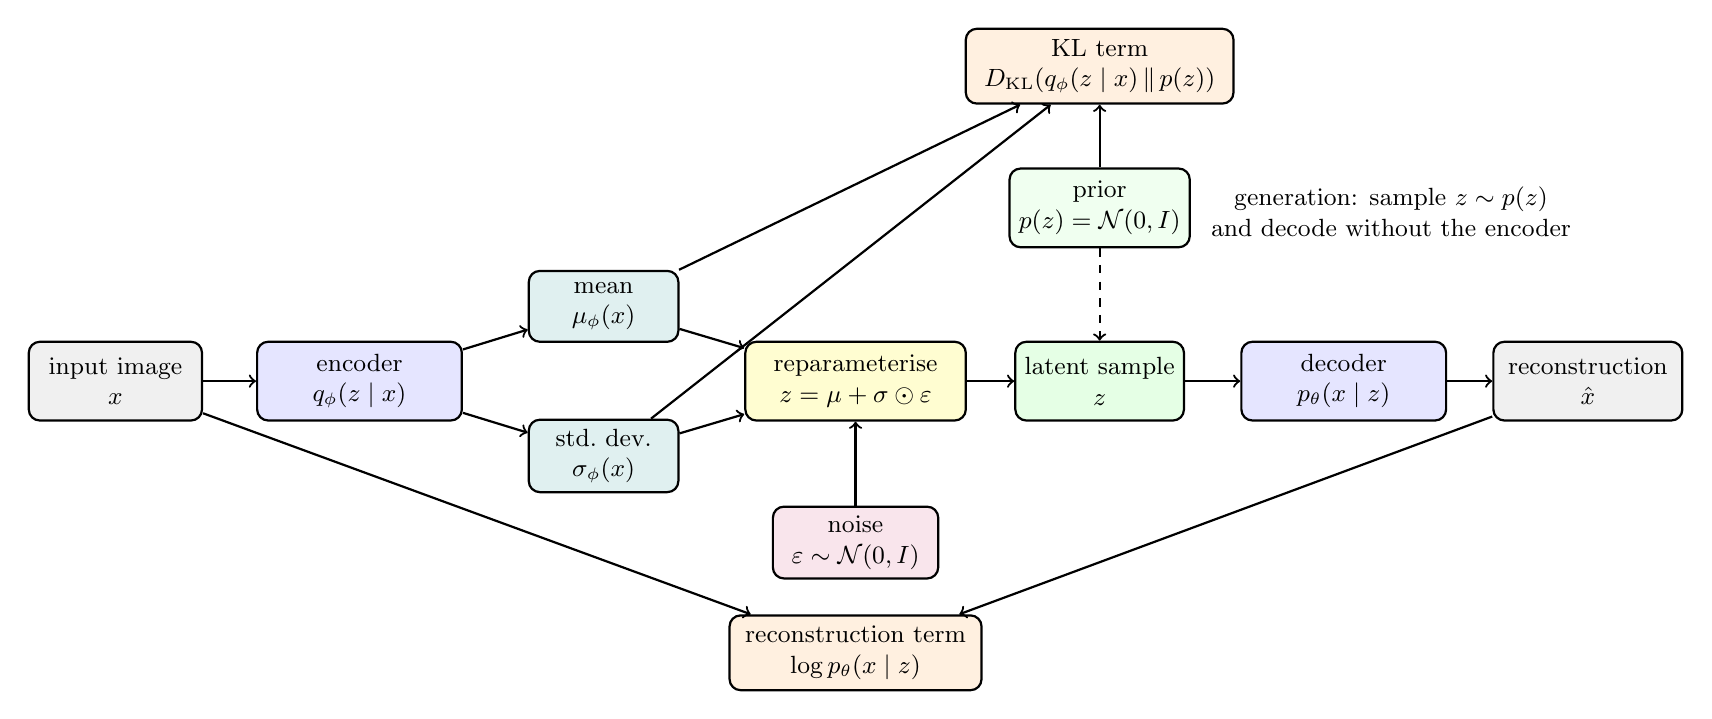
\begin{tikzpicture}[font=\small]
        \node[draw, rounded corners, thick, align=center, minimum width=2.2cm,
            minimum height=1.0cm, fill=gray!12] (x) at (0,0) {input image\\$x$};
        \node[draw, rounded corners, thick, align=center, minimum width=2.6cm,
            minimum height=1.0cm, fill=blue!10] (enc) at (3.1,0) {encoder\\$q_\phi(z \mid x)$};
        \node[draw, rounded corners, thick, align=center, minimum width=1.9cm,
            minimum height=0.9cm, fill=teal!12] (mu) at (6.2,0.95) {mean\\$\mu_\phi(x)$};
        \node[draw, rounded corners, thick, align=center, minimum width=1.9cm,
            minimum height=0.9cm, fill=teal!12] (sigma) at (6.2,-0.95) {std.\ dev.\\$\sigma_\phi(x)$};
        \node[draw, rounded corners, thick, align=center, minimum width=2.8cm,
            minimum height=1.0cm, fill=yellow!18] (reparam) at (9.4,0)
            {reparameterise\\$z = \mu + \sigma \odot \varepsilon$};
        \node[draw, rounded corners, thick, align=center, minimum width=2.1cm,
            minimum height=0.9cm, fill=purple!10] (eps) at (9.4,-2.05)
            {noise\\$\varepsilon \sim \mathcal{N}(0, I)$};
        \node[draw, rounded corners, thick, align=center, minimum width=2.1cm,
            minimum height=1.0cm, fill=green!10] (z) at (12.5,0) {latent sample\\$z$};
        \node[draw, rounded corners, thick, align=center, minimum width=2.6cm,
            minimum height=1.0cm, fill=blue!10] (dec) at (15.6,0) {decoder\\$p_\theta(x \mid z)$};
        \node[draw, rounded corners, thick, align=center, minimum width=2.4cm,
            minimum height=1.0cm, fill=gray!12] (xhat) at (18.7,0) {reconstruction\\$\hat{x}$};
        \node[draw, rounded corners, thick, align=center, minimum width=2.2cm,
            minimum height=1.0cm, fill=green!6] (prior) at (12.5,2.2)
            {prior\\$p(z) = \mathcal{N}(0, I)$};
        \node[draw, rounded corners, thick, align=center, minimum width=3.2cm,
            minimum height=0.95cm, fill=orange!12] (reconloss) at (9.4,-3.45)
            {reconstruction term\\$\log p_\theta(x \mid z)$};
        \node[draw, rounded corners, thick, align=center, minimum width=3.4cm,
            minimum height=0.95cm, fill=orange!12] (klloss) at (12.5,4.0)
            {KL term\\$D_{\mathrm{KL}}(q_\phi(z \mid x)\,\|\,p(z))$};

        \draw[->, thick] (x) -- (enc);
        \draw[->, thick] (enc) -- (mu);
        \draw[->, thick] (enc) -- (sigma);
        \draw[->, thick] (mu) -- (reparam);
        \draw[->, thick] (sigma) -- (reparam);
        \draw[->, thick] (eps) -- (reparam);
        \draw[->, thick] (reparam) -- (z);
        \draw[->, thick] (z) -- (dec);
        \draw[->, thick] (dec) -- (xhat);
        \draw[->, thick] (x) -- (reconloss);
        \draw[->, thick] (xhat) -- (reconloss);
        \draw[->, thick] (mu) -- (klloss);
        \draw[->, thick] (sigma) -- (klloss);
        \draw[->, thick] (prior) -- (klloss);
        \draw[dashed, thick, ->] (prior) -- (z);

        \node[align=center] at (16.2,2.15) {generation: sample $z \sim p(z)$\\and decode without the encoder};
    \end{tikzpicture}%
    }
    \caption{Overview of VAE training and generation. The encoder produces an approximate
    posterior over latent codes, the reparameterisation step turns that posterior into a
    differentiable sample, and the decoder maps the sample back to the image space.
    Training combines reconstruction quality with a KL penalty toward the Gaussian prior.
    At generation time, a fresh sample from the prior can be decoded directly.}
    \label{fig:vae_architecture}
\end{figure}

More formally, a VAE~\citep{kingma2013auto} defines a latent-variable generative model
$p_\theta(x) = \int p_\theta(x \mid z)\,p(z)\,\mathrm{d}z$, where $p(z) = \mathcal{N}(0, I)$
is a standard Gaussian prior and $p_\theta(x \mid z)$ is a learned decoder. Because the
marginal likelihood is intractable, training maximises the evidence lower bound (ELBO):
\begin{equation}
    \mathcal{L}_{\mathrm{VAE}}(\theta, \phi; x)
    = \underbrace{\mathbb{E}_{q_\phi(z \mid x)}\!\left[\log p_\theta(x \mid z)\right]}_{\text{reconstruction}}
    -\underbrace{D_{\mathrm{KL}}\!\left(q_\phi(z \mid x)\,\|\,p(z)\right)}_{\text{regularisation}},
    \label{eq:elbo}
\end{equation}
where $q_\phi(z \mid x) = \mathcal{N}(\mu_\phi(x), \mathrm{diag}(\sigma^2_\phi(x)))$ is the
encoder's approximate posterior. The first term rewards reconstructions that explain the
observed data; the second keeps the posterior close to the prior so that prior samples
remain meaningful and neighbouring latent codes decode to similar outputs. The
reparameterisation trick $z = \mu_\phi(x) + \sigma_\phi(x) \odot \varepsilon$,
$\varepsilon \sim \mathcal{N}(0, I)$, expresses stochastic sampling as a differentiable
transformation of parameter-free noise, enabling end-to-end optimisation with standard
backpropagation. This smooth, sampleable latent space is precisely the property Phase~2
exploits: composition by latent substitution is only coherent when the latent geometry
organises factors in a predictable way.

\subsection{Disentangled Representations}

A representation is \emph{disentangled} if each latent dimension encodes at most one
ground-truth factor of variation, and changing one dimension changes the corresponding
attribute without affecting others~\citep{disentengaled_representation_learning,
on_disentangled_representation_learning}. This property is desirable for compositional
generation because it supports surgical factor substitution: given a reference image and a
donor, swapping the dimension encoding orientation should change orientation alone, leaving
scale and content intact.

$\beta$-VAE~\citep{Higgins2016betaVAELB} encourages disentanglement by scaling the KL term
in Equation~\ref{eq:elbo} by $\beta > 1$, creating a stronger information bottleneck that
pushes the encoder toward axis-aligned, factorial posteriors. FactorVAE~\citep{disentangling_by_factorising}
replaces the KL coefficient with a Total Correlation penalty $\gamma\,\mathrm{TC}(q(z))$,
where $\mathrm{TC}(q(z)) = D_{\mathrm{KL}}(q(z)\,\|\,\prod_j q(z_j))$ measures the excess
dependence of the aggregate posterior beyond its marginals. Both approaches rely on
statistical independence pressure within a single shared latent code $z \in \mathbb{R}^d$,
which works well when the generative factors are sampled independently. Under correlated
training data, however, the model can exploit the correlation between factors as a
prediction shortcut, and regularisation pressure alone cannot prevent this. Locatello et
al.~\citep{locatello2019challenging} showed that unsupervised disentanglement is
fundamentally unidentifiable without inductive bias: with enough random seeds, any method
can appear to disentangle, making the result unreliable in practice. This is the failure
mode that motivates the supervised and structurally partitioned regimes in Phase~2.

\paragraph{Measuring disentanglement: DCI.}
The DCI framework~\citep{eastwood2018framework} quantifies representation quality through
three complementary scores derived from a factor-importance matrix $R \in \mathbb{R}^{d
\times K}$, where $d$ is the latent dimensionality and $K$ is the number of known
ground-truth factors. Each entry $R_{jk}$ measures how strongly latent dimension $j$
contributes to predicting factor $k$, estimated from a gradient-boosted regressor trained
on the deterministic encoder mean $\mu_\phi(x)$. Column-normalising $R$ gives
$\tilde{R}_{jk} = R_{jk} / \sum_{k'} R_{jk'}$, the share of dimension $j$'s importance
explained by factor $k$. Row-normalising gives $\hat{R}_{jk} = R_{jk} / \sum_{j'}
R_{j'k}$, the share of factor $k$'s signal captured by dimension $j$.
\textbf{Disentanglement} ($\mathcal{D}$) measures whether each latent dimension encodes
at most one factor:
\begin{equation}
    \mathcal{D} = \sum_{j=1}^{d} \rho_j\!\left(1 - H_K(\tilde{R}_{j\cdot})\right),
    \qquad
    \rho_j = \frac{\sum_k R_{jk}}{\sum_{j'}\sum_k R_{j'k}},
    \label{eq:dci_d}
\end{equation}
where $H_K(p) = -\sum_k p_k \log_K p_k$ is Shannon entropy normalised by $\log K$ and
$\rho_j$ weights each dimension by its total importance so that uninformative dimensions
contribute negligibly. \textbf{Completeness} ($\mathcal{C}$) measures whether each factor
is captured by a small number of dedicated dimensions:
\begin{equation}
    \mathcal{C} = \frac{1}{K}\sum_{k=1}^{K}\!\left(1 - H_K(\hat{R}_{\cdot k})\right).
    \label{eq:dci_c}
\end{equation}
\textbf{Informativeness} ($\mathcal{I}$) is the mean held-out prediction accuracy of the
$K$ regressors. Both $\mathcal{D}$ and $\mathcal{C}$ equal one at perfect disentanglement
and zero when importance is spread uniformly; $\mathcal{I}$ confirms the factors are
recoverable at all, making low $\mathcal{D}$ or $\mathcal{C}$ interpretable as entanglement
rather than collapse.

\subsection{Weakly Supervised Disentanglement and Structural Partitioning}

Because unsupervised disentanglement is unreliable under correlated data, two complementary
remedies have been proposed: label-based factor supervision and structural latent
partitioning.

\paragraph{Label-supervised auxiliary heads.}
A lightweight approach introduced by Locatello et al.~\citep{locatello2020weakly} and
formalised in several attribute-disentanglement works is to attach training-only predictor
heads to the deterministic encoder mean $\mu_\phi(x)$. For each known factor $k$, a small
MLP $g_k$ is trained with a cross-entropy or regression loss against the ground-truth label
$y_k$. The heads are discarded at inference, leaving only the encoder's learned
representation. Attaching supervision to $\mu_\phi(x)$ rather than the stochastic sample
$z$ makes the gradient deterministic and reduces variance, consistent with how
disentanglement is evaluated~\citep{eastwood2018framework,
challeau2019challenging}. Traeuble et al.~\citep{traeuble2021disentangled} showed that
under correlated training data such weak supervision partially recovers factor separation
that independence-based objectives miss entirely.

\paragraph{Gradient reversal for adversarial exclusion.}
Correct-head supervision pushes a factor \emph{into} the intended latent region, but it
does not actively prevent that factor from also leaking into a different region. Ganin and
Lempitsky~\citep{ganin2015unsupervised, ganin2016domain} introduced the gradient reversal
layer (GRL) to remove a nuisance attribute from a representation adversarially: the GRL
is the identity in the forward pass, so the attached classifier receives real activations
and produces a real loss; in the backward pass it multiplies the incoming gradient by
$-\lambda$ before passing it to the encoder. Without GRL, minimising a cross-entropy loss
on classifier $g$ would encourage the encoder to make the attribute \emph{more} predictable
from the wrong region; with GRL, the reversed gradient instructs the encoder to make it
\emph{less} predictable, while the classifier's own weights remain unreversed and continue
improving at detecting whatever residual leakage survives. This minimax dynamic drives
cross-attribute leakage toward zero at convergence. Scaramuzzino et
al.~\citep{attribute_disentanglement} applied exactly this mechanism to attribute-specific
latent separation in fashion retrieval, demonstrating that correct-head supervision paired
with GRL-mediated wrong-head suppression produces cleaner factor isolation than supervision
alone.

\paragraph{Structural latent partitioning: SepVAE.}
SepVAE~\citep{louiset2024sepvae} showed that in a contrastive setting --- a background
cohort of healthy subjects and a target cohort carrying a specific pathology --- the most
reliable way to separate common from pathology-specific variation is to allocate each to
its own latent partition rather than hoping regularisation produces the separation within a
shared code. The model defines a common code $z_c$ shared across both cohorts and a
salient code $z_s$ specific to the target, with generative constraints tied to the
background/target asymmetry enforcing that the common code captures normal anatomy and
$z_s$ captures the pathological deviation. The key insight generalises beyond the medical
domain: structural allocation removes the possibility of entanglement that regularisation
can only penalise after it occurs.
